\documentclass[12pt]{article}
\usepackage[utf8]{inputenc}
\usepackage{amsmath}
\usepackage{graphicx}
\title{CS 470 Spring 2011 \\
     Project 1}
\author{Colby Blair}
\date{Due February 18th, 2011}
\begin{document}
\maketitle
\begin{abstract}
In Artificial Intelligence, we can test intelligent agents on their ability to navigate maps to reach a goal position. For each position, there is a choice of options that we can take, and how process these options depends on which search we choose. With each step, our new possible routes increases exponentially. The search algorithm must be able to handle all these possible routes one by one, and build routes efficiently. This report will test the Breadth First Search, discuss the methodology, and highlight the pros and cons of this type of search.
\\ \\
With all searches, there is a tradeoff between best Path Cost, Time Complexity, and Space Complexity. If one needs absolute best (least) Path Cost,  Lowest Cost Search is the best across all map systems. Iterative Deepening By Cost Search finds the lowest cost path and is slightly better than Lowest Cost Search, but its Time Complexity eclipses all other searches. A* searches can be better than all searches, but you have to develop really good heuristics (estimates on future cost). This is tough to do for all possible maps, so without a lot of work in heuristics, Lowest Cost Search is the best bet all around.
\end{abstract}
\pagebreak

\tableofcontents



\pagebreak

\section{Introduction}
Searching through maps comes down to 3 factors to trade off: Path Cost, Time Complexity (time spent searching), and Space Complexity (memory of past and next locations). Some searches find a good combonation of all three, but if a search is needed that finds the optimum path, we have to pay a price.

\section{Path Tracing}
An extra feature to searching is to trace the path an individual took to get to the location. There are several ways to do this. The way the search did this here is each node on the Value Matrix had a Parent Pointer. This pointer was set to Null initially. Then, whenever a node (or cell) was added to the frontier queue, the corresponding cell node on the Value Matrix had its parent pointer set to the corresponding Value Matrix cell node of the node that added.
	\\ \\
For example, in the figures for Breadth Search below, when cell node 'start' added cell node 3 to the frontier queue, Value Matrix cell node 3's parent was set to Value Matrix cell node 'start'. Since cell node 3 could only ever be added once, it will only ever have its parent set once. Thus, a route back to the cell node 'start' will always be found anywhere in the explored Value Matrix.

\section{Breadth First Search}
	\subsection{Procedure}
	Consider a map like the following:
	\\
	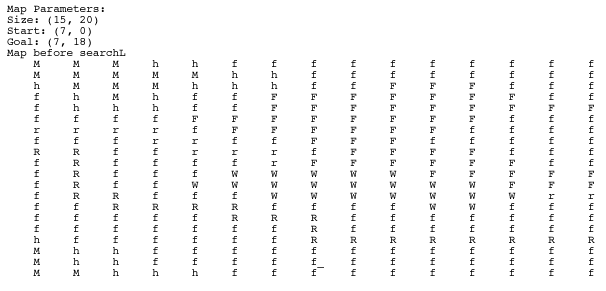
\includegraphics[width=120mm,height=60mm]{images/init_map.png}
	\\
	The search starts at cell x = 7, y = 0. Each cell has a cost signified by a character (R = low cost road, M = high cost mountain), but Breadth First Search does not care. It will simply find the shortest distance to the goal (there may be multiple that are equal). The only time this algorithm considers cost is when it is going off the side of the map or going into W (water), both of which have an invalid cost of 0 and are not considered.
	\\ \\
	This Breadth First Search uses 3 data structures: a Frontier Queue, an Explored List, and a Value Matrix. The only technical notes past these is that the Value Matrix is a matrix (or 2 dimensional array) of 'node' classes. Each 'node' class has members name, val, x, and y (where val equals the cost of the cell). Value\_Matrix[0][0] then equals node('M',10,0,0), etc. Later we will see that each cell node also has a node parent pointer, but ignore this for now.
 
	Let's consider our start section of the map:
	\begin{center} 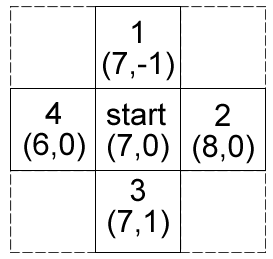
\includegraphics[width=60mm]{images/init_pos.png} \end{center}
	Cells above are labeled in the order the algorithm adds them to a queue.
	\begin{enumerate}
		\item 'start' is added.
		\item while the front of the queue is not the goal:
		\begin{enumerate}
			\item front's neighbors are added to the end of the queue
			\item front is popped from the queue
		\end{enumerate}
	\end{enumerate}
	So each iteration would look something like the following:
	\\ \\
	\begin{center}
		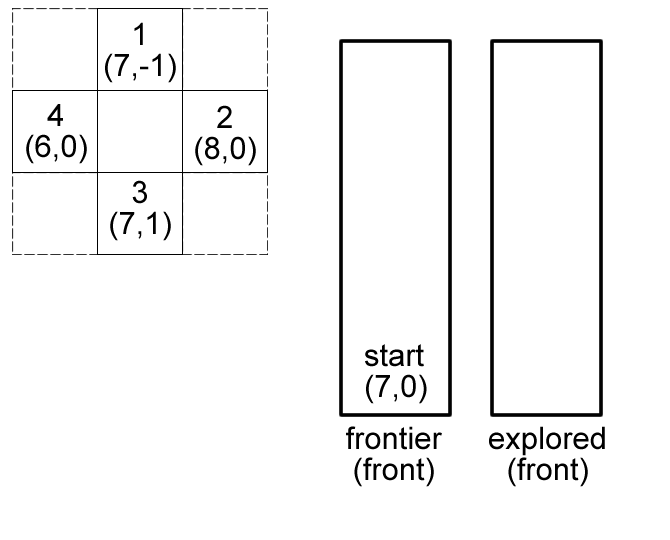
\includegraphics[width=60mm]{images/breadth/pos01.png}
		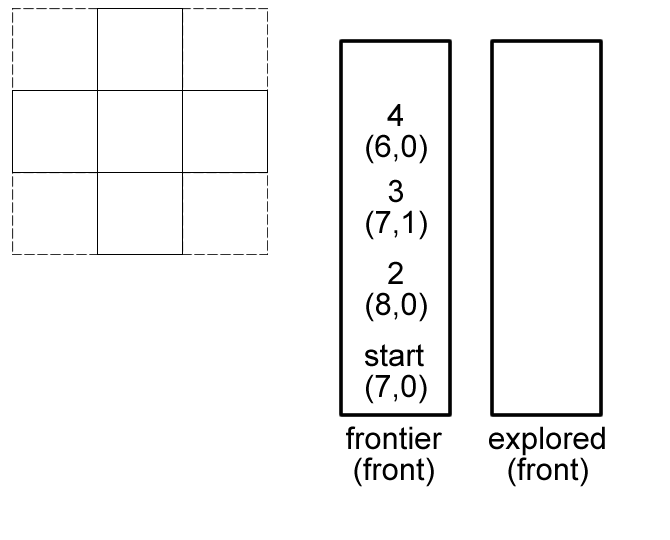
\includegraphics[width=60mm]{images/breadth/pos02.png}
		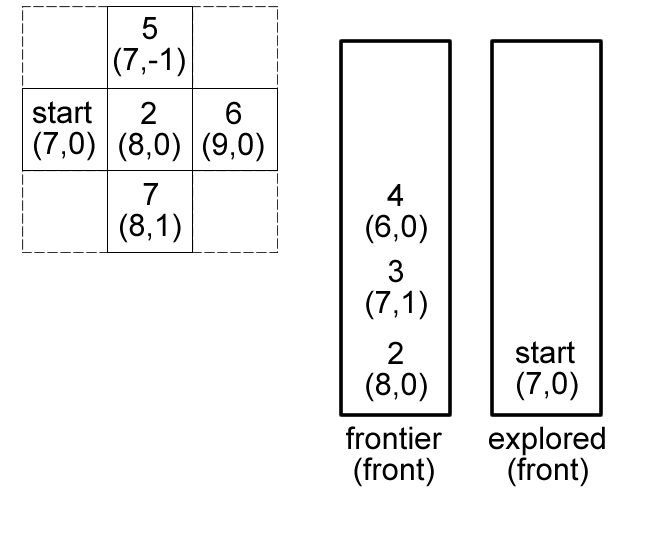
\includegraphics[width=60mm]{images/breadth/pos03.png}
		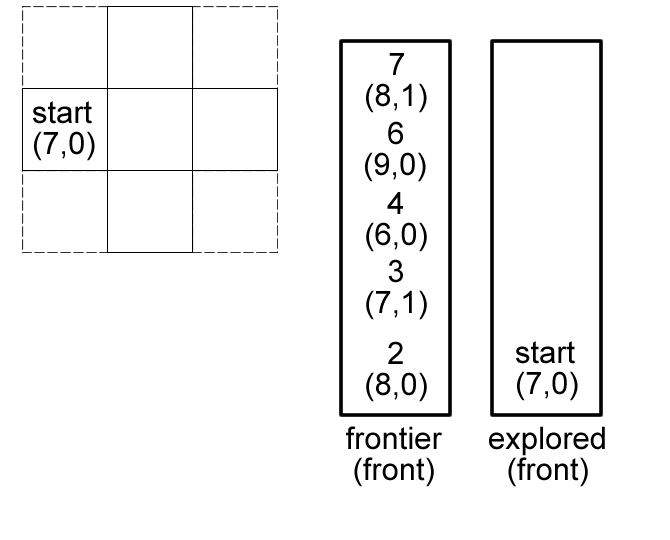
\includegraphics[width=60mm]{images/breadth/pos04.png}
		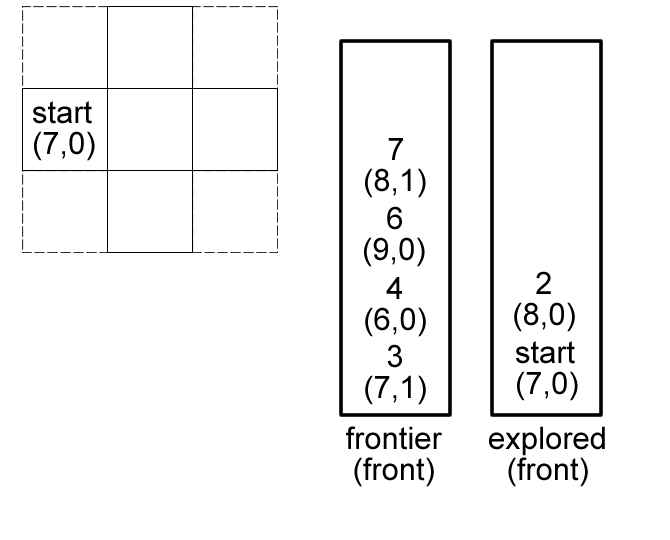
\includegraphics[width=60mm]{images/breadth/pos05.png}
	\end{center}

	This would continue on until the node (or cell) on the front of frontier queue was the goal. Notice that the search does not add nodes outside the bounds of the map or matrix (i.e. nodes 1 and 5 above). Also, nodes (or cells) that already exist in the explored list are not re-added to the frontier list.

	\subsection{Procedure Summary}
	This search is called a Breadth First Search because at every cell, there is a decision tree of possible new cells to move to. When the search processes every neighbor cell first before processing those neighbor cells' neighbors, the search has covered the breadth of the top level of the decision tree before moving on. In contrast, if the search was at the 'start' cell, processed cell 3 from above, and then processed all of cell 3's neighbors before looking at cell 4, the search would be searching as a Depth First Search.
	\\ \\
	The Depth First search would be searching each possible 1st neighbor until the last possible neighbor, and then backing up from the bottom of the decision tree. Cell 4 above wouldn't get considered until every possible path from cell 3 was exhausted with no route to the goal.

	\subsection{Completeness, Efficiency (Cost and Path Length), and Complexity}
	The Breadth First Search is a \textbf{Complete} search, meaning it will find the goal if one exists. In \textbf{Efficiency}, it will always find the shortest path, but almost never find the least cost path.  Thus, it will find the shallowest solution in the decision tree. The \textbf{Time Complexity} (or time it takes to find the goal) is $\approx B^{d}$, or about the number of each neighbor a cell could have to the power of the max depth of the decision tree. The \textbf{Space Complexity} (memory used, or storage all new neighbors to the frontier queue) is $\approx B^{d}$.
	\\ \\
	This search is advantageous to the Depth First Search, which is only sometimes complete (only when the depth is finite). This search will also find the shallowest solution (shortest path), which is not gaurenteed or even likely for Depth First Search. Depth first search will almost always have less Time Complexity (quicker) with an upper bound of $B^{d}$, and will have less Space Complexity (uses less memory). In practicality, very big maps would have to use Depth First Search for the Complexity reasons.

	\subsection{Program Output}
	The final output of the Breadth First Search is:
	\\
	\begin{center}
		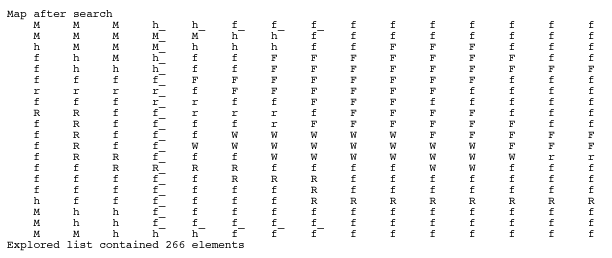
\includegraphics[width=120mm,height=60mm]{images/breadth/final_breadth_map.png}
	\end{center}
	We can see that this search takes the straightest path over until the 'W' water barrier is out of the way. The search goes straight down towards the goal, and then once parallel, cuts straight back across. This is the shortest path on our discrete map of cells. It is in now way the least cost path, but it is the straightest, considering the impassable 'W' water barrier.

	\subsection{Breadth Conclusion}
	The Breadth First Search found the straightest path, but at a high Space Complexity / memory price. The frontier explored list contained 266 cell nodes, the majority of the 15 x 20 map (300 cell nodes). This Space Complexity on a larger map could be a big issue, and a different search algorithm may be needed.


\section{Lowest Cost Search}

	\subsection{Procedure}
	Let's consider again the start section of the map:
	\begin{center} 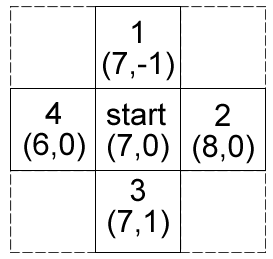
\includegraphics[width=60mm]{images/init_pos.png} \end{center}

	The process for Lowest Cost is as follows:
	\begin{enumerate}
		\item while goal cell node is not at the front of the frontier list
		\begin{enumerate}
			\item if the cell node at the front of the frontier list is not in the exlpored list:
				\begin{enumerate}
					\item add the front of the frontier list to the explored list
					\item pop the front of the frontier list
					\item push the neighbors of the popped cell node onto the front of the frontier list
					\begin{itemize}
						\item neighbors are sorted from lowest cost to  cost
						\item the neigbor with the lowest cost will be on the front of the frontier list
					\end{itemize}
				\end{enumerate}
			\item else pop the front of the frontier list
		\end{enumerate}
	\end{enumerate}

	So each iteration would look like the following: \\ \\
	\begin{center}
		\includegraphics[width=60mm]{images/cost/pos01.png}
		\includegraphics[width=60mm]{images/cost/pos02.png}
	\end{center}
	\begin{center}
		\includegraphics[width=60mm]{images/cost/pos03.png}
		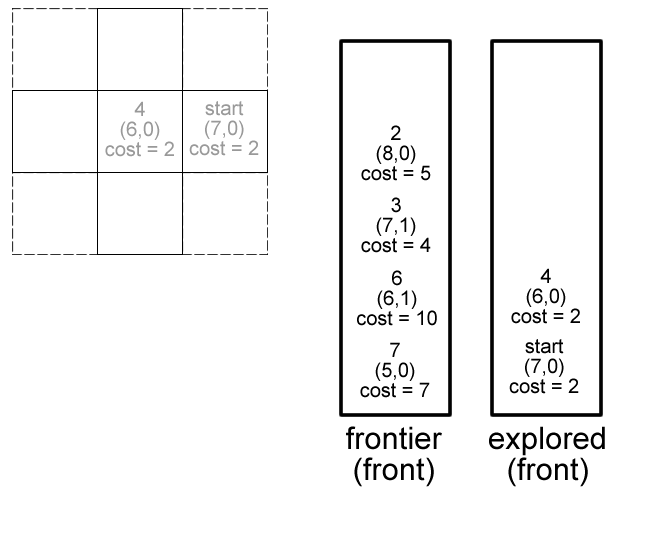
\includegraphics[width=60mm]{images/cost/pos04.png}
	\end{center}
	\begin{center}
		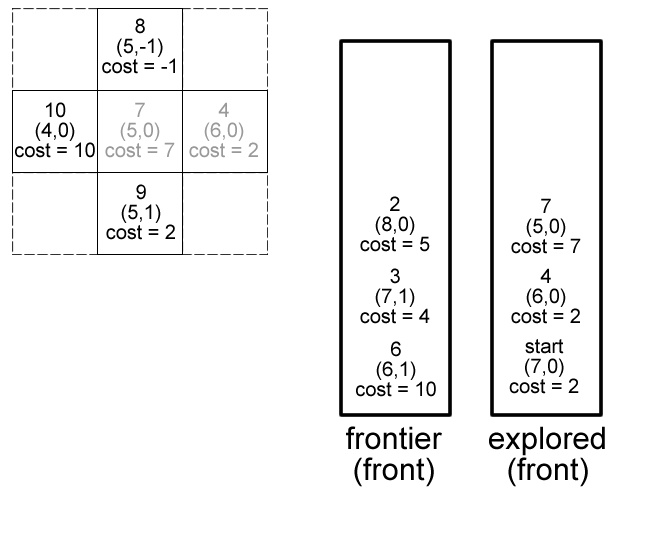
\includegraphics[width=60mm]{images/cost/pos05.png}
	\end{center}

	\subsection{Procedure Summary}
	Search by Lowest Cost is a Depth First Search by Cost. It considers a cell node's neighbors, and picks the lowest cost cell node of those neighbors. It then looks at the lowest cost of that neighbor's neighbors, and pursues through the depth of that decision tree until the end. If it finds the goal, it finishes. If it hits a dead end, it returns to the previous neighbors and considers the next lowest cost, again until it finds a goal, or again if it hits a dead end, it goes back up the decision tree and considers the next lowest cost neighbors of the next highest level.

	\subsection{Completeness, Efficiency (Cost and Path Length), and Complexity}
	Since this search is Depth First, it doesn't offer \textbf{Completeness} unless the map is limited. In our example maps, it is, but real world maps may be intractable. Since Least Cost is Depth First, it probably won't find the most \textbf{Efficient} path. It probably creates a longer \textbf{Path Length} than Breadth and Depth First, but a lower \textbf{Cost} than Depth and Breadth. \textbf{Time Complexity}  is $B^D$ as an upper bound, but usually does better. \textbf{Space Complexity} is $B * D$, which is this search's main advantage over other searches. Its Space Complexity is considerably better then many other searches.

	\subsection{Program Output}
	The final output of the Search is:
	\\
	Explored:
	\begin{center}
		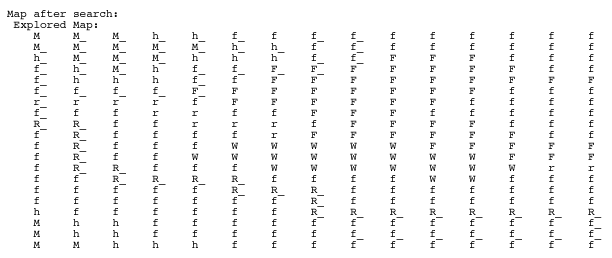
\includegraphics[width=120mm,height=60mm]{images/cost/final_map_explored.png}
	\end{center}

	\pagebreak

	Path:
	\begin{center}
		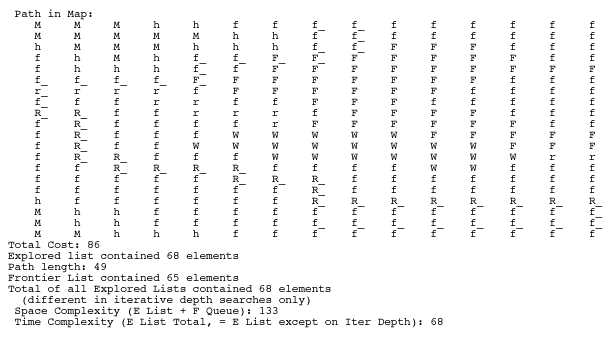
\includegraphics[width=120mm,height=60mm]{images/cost/final_map_path.png}
	\end{center}

	\subsection{Lowest Cost Conclusion}
	Lowest Cost Search is a reasonably good search to pick; it gets the next best cost path for a lot less Time Complexity. It could potentially be beat all around by A* Search with good heuristics, but it's algorithm has no dependency on any system, and performs with less Complexity than A*'s worst case scenario

\section{Iterative Deepening By Cost Search}

	\subsection{Procedure}
	The process for Iterative Deepening is simply the Least Cost with Max Cost incremented until the goal is reached: 
	\\ \\
	max cost = 2
		\begin{enumerate}
			\item while goal cell node is not at the front of the frontier list
			\begin{enumerate}
				\item if the cell node at the front of the frontier list is not in the explored list AND its cost $<=$ max cost
					\begin{enumerate}
						\item add the front of the frontier list to the explored list
						\item pop the front of the frontier list
						\item push the neighbors of the popped cell node onto the front of the frontier list
						\begin{itemize}
							\item neighbors are sorted from lowest cost to highest cost
							\item the neigbor with the lowest cost will be on the front of the frontier list
						\end{itemize}
					\end{enumerate}
				\item else pop the front of the frontier list
				\item if the frontier list is empty, or if the frontier list is empty AND cost $>$ max depth
				\begin{enumerate}
					\item clear out the frontier list, leaving only the start cell node
					\item clear out the current explored list
					\item increment max cost by 1
				\end{enumerate}
			\end{enumerate}
		\end{enumerate}

	So a process with a \textbf{max cost of 7} would look like: \\ \\
	\begin{center}
		\includegraphics[width=60mm]{images/icost/pos01.png}
		\includegraphics[width=60mm]{images/icost/pos02.png}
	\end{center}
	\begin{center}
		\includegraphics[width=60mm]{images/icost/pos03.png}
		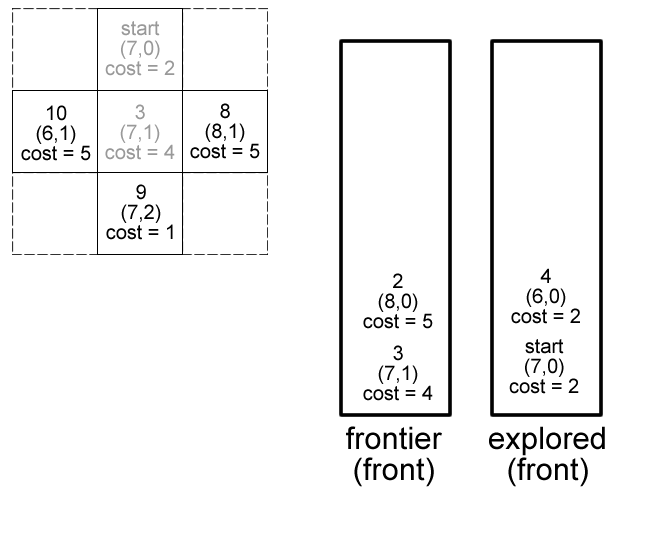
\includegraphics[width=60mm]{images/icost/pos04.png}
	\end{center}
	\begin{center}
		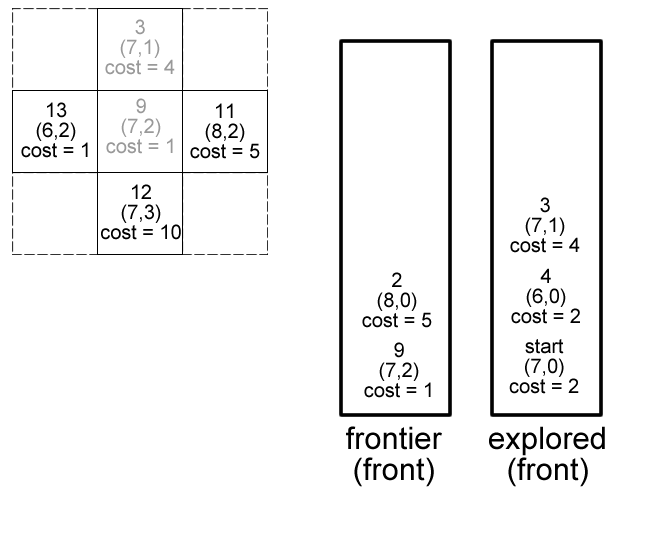
\includegraphics[width=60mm]{images/icost/pos05.png}
	\end{center}

	\subsection{Procedure Summary}
	Iterative Deepening by Cost was very similar to Search By Cost, except it placed an 'artifical' max cost that. The advantage to this was that it would stop at the max cost depth, and then explore its neighbors, and then all the neighbors above the max cost depth in the search tree. And then the search would explore those neighbors' children back down to the max cost depth. If the whole tree didn't have the goal, then the max cost would be incremented, and a whole other level of children were available on the bottom of the tree. 
	\\ \\
	The advantage is that the search tends to look around much better in its surroundings and explore good low cost paths. The disadvantage is that everytime the max cost depth is increased, the whole search has to start from the top of the search tree (or the start cell node). 

	\subsection{Completeness, Efficiency (Cost and Path Length), and Complexity}
	Iterative Deepening by Cost was probably the best all around search. It found the best path in my tests, although a A* Search with a great heuristic could beat it. It is \textbf{Complete}, like Breadth First; it is like a bottom-up Breadth Search in a way. It is gauranteed to find the most \textbf{Cost} \textbf{Efficient} path (unlike Breadth First), but not likely the shortest \textbf{Path Length}. 
	\\ \\
	The search's \textbf{Space Complexity} is:
		\begin{equation}
			S_c =|Least Cost Path| + |Last Iteration Explored List| <= B * D << B^D
		\end{equation}
	 -by far better than all other searches, with possibly the exception of an A* Search with a really great Heuristic. The only disadvantage is that the \textbf{Time Complexity} is $ {(i - 1) * B^D} + |Least Cost Path|$ where i is how many iterations of the max cost depth it took before the goal was found. This is considerably larger than even a Depth First Search.

	\subsection{Program Output}
	The final output of the Search is:
	\\
	Explored Map
	\begin{center}
		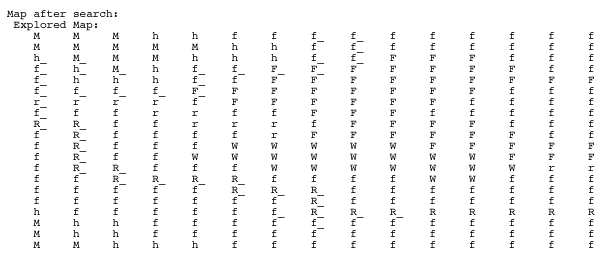
\includegraphics[width=120mm,height=60mm]{images/icost/final_map_explored.png}
	\end{center}

	\begin{center}
		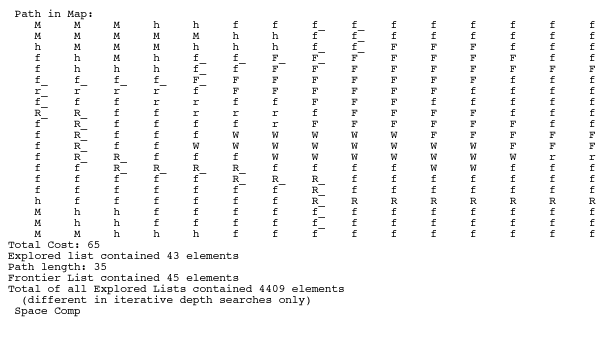
\includegraphics[width=120mm,height=60mm]{images/icost/final_map_path.png}
	\end{center}

	\subsection{Iterative Deepening by Cost Conclusion}
	Even though this search's Time Complexity was so enormous, it found the best path for the lowest Space Complexity. This may often be the case in real life. If the answer needs to be quicker, then it will probably not be as Efficient or it may take much more Space Complexity. But if one just needs an answer, this search may be the best until the Time Complexity or map is untractable.

\section{A* Search With Multiple Heuristics}

	\subsection{Procedure}
	\begin{enumerate}
		\item while the goal cell node is not on the front of the frontier list
		\begin{enumerate}
			\item if the front of the frontier list is not in the explored list
				\begin{enumerate}
					\item add the front of the frontier list to the explored list
					\item pop the front of the frontier list
					\item push the neighbors of the popped cell node onto the front of the frontier list
					\begin{itemize}
						\item neighbors are sorted from lowest cost to highest cost
						\item the neigbor with the lowest cost will be on the front of the frontier list
						\item cost is determined by the cell node cost + one of two heuristics (see below)
					\end{itemize}				
				\end{enumerate}
			\item else pop the front of the frontier list
		\end{enumerate}	
	\end{enumerate}

	The process isn't easy to illustrate without looking at the entire graph, bu isn't difficult to understand when reading about the heuristics while looking at the output.

	\subsection{Heuristics}
	For heuristics to find the optimal path, they must never overestimate (is admissable). Each of these heuristics underestimate the true cost, but try to approach true cost.
 
		\subsubsection{H1 - Manhattan Distance}
		The first heuristic that the program used was calculating Manhattan Distance. For each cell node, its heuristic was the length of the shortest possible path to the goal. This underestimated true cost by saying each future node on the Manhattan Path would have a cost of 1.
	
		\subsubsection{H2 - Cost Guilt By Association}
		The second Heuristic tried to judge a bad neighborhood to explore by judging a cell node by it immediate neighbors (4 cell nodes surrounding it left, right, top and bottom). If a cell node was in a high cost neighborhood, the heuristic was high. This heuristic overestimates when there are single high cost cell node outliers, but in more continuous landscape tends not to overestimate, since the neighbors will be likely paths.

	\subsection{Procedure Summary}
	H1 performed better than H2, despite seeming to be dumber. Its ability to underestimate more seemed to help it. H2 should have perhaps taken the least cost of a cell node's neighbors instead of an average. 

	\subsection{Completeness, Efficiency (Cost and Path Length), and Complexity}
	A* was a Depth First Search with a lookahead, so it was not at all \textbf{Complete}. With better heuristics, it could surpase Iterative Deepening by Cost's \textbf{Space Complexity} as $ S_c =  |Least Cost Path| + |Length of Explored List|$, each of which would be less. Both H1 and H2 have a much better \textbf{Time Complexities} $T_c = |Length of Explored List| $. Both H1 and H2 lost slightly to Breadth Search in Cost, but make it up in considerably less complexity.

	\pagebreak

	\subsection{Program Output}
	The final output of the A* H1 Search is:
	\\
	Explored:
	\begin{center}
		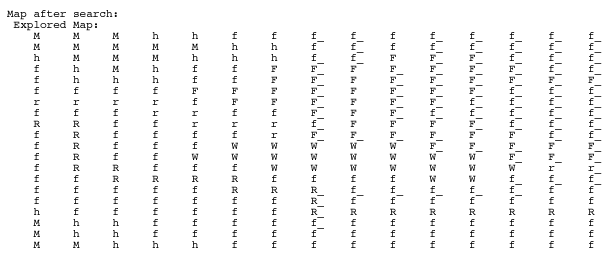
\includegraphics[width=120mm,height=60mm]{images/ah1/final_map_explored.png}
	\end{center}
	Path:
	\begin{center}
		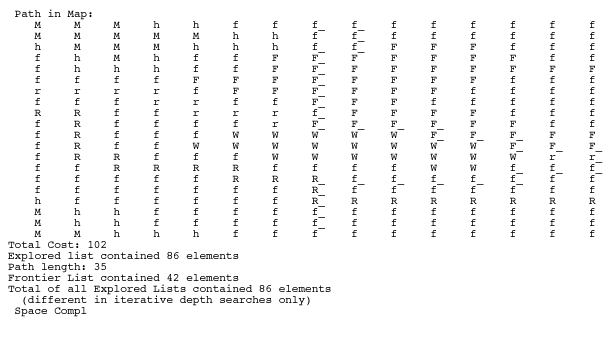
\includegraphics[width=120mm,height=60mm]{images/ah1/final_map_path.png}
	\end{center}

	\pagebreak

	The final output of the A* H2 Search is:
	\\
	Explored:
	\begin{center}
		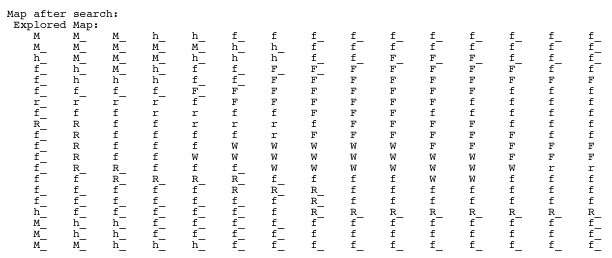
\includegraphics[width=120mm,height=60mm]{images/ah2/final_map_explored.png}
	\end{center}
	Path:
	\begin{center}
		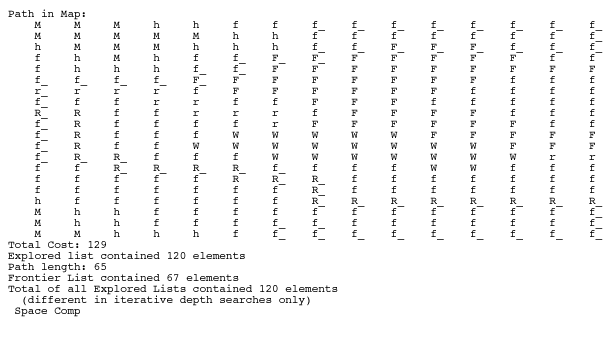
\includegraphics[width=120mm,height=60mm]{images/ah2/final_map_path.png}
	\end{center}

	\pagebreak

	\subsection{A* Search Conclusion}
	A* Search is a good search, and tends to be the right middle ground between Time Complexity versus Space Complexity. With really good heuristics, it could become better. It is tough to make a good heuristic that is independent of the sampled systems, and I was only able to try with mild success.

\section{Algorithm Comparison}
	\begin{center}
		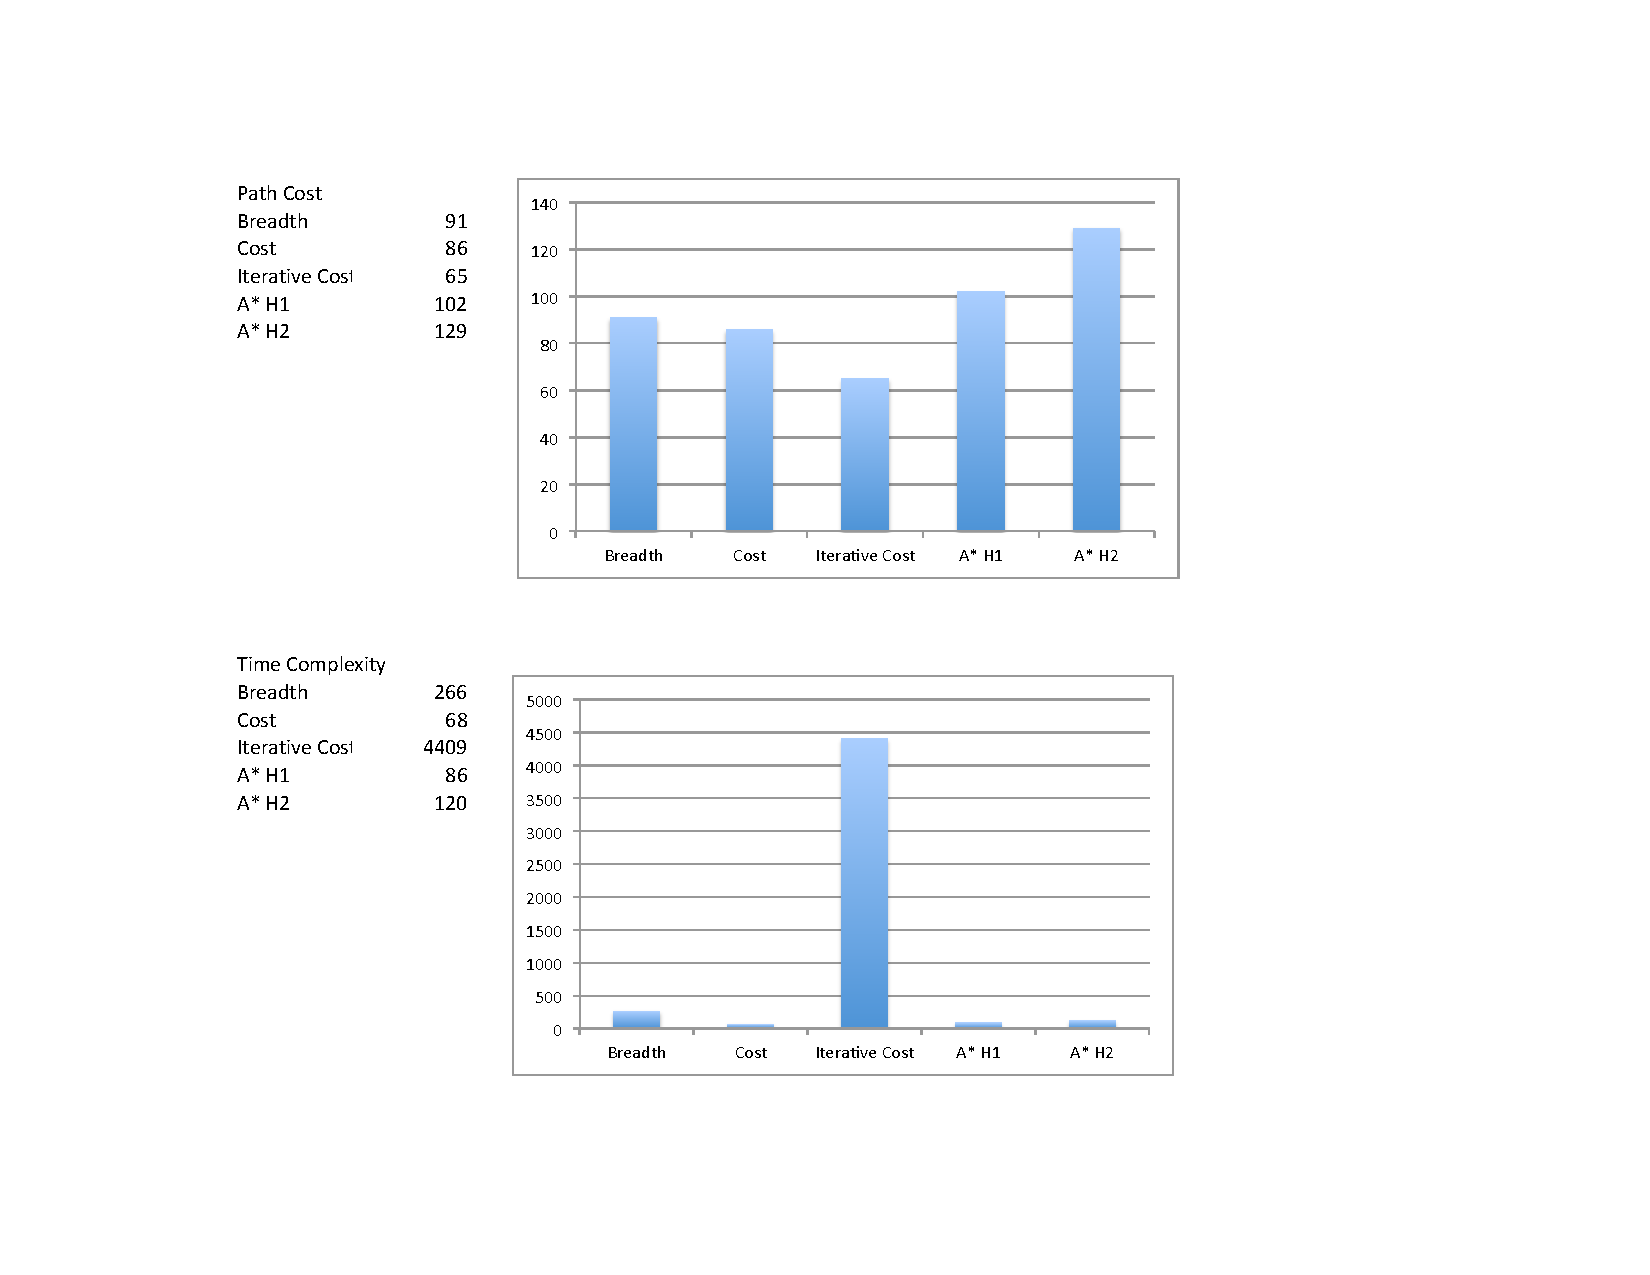
\includegraphics[width=150mm,height=120mm]{images/results1.pdf}
	\end{center}
	\begin{center}
		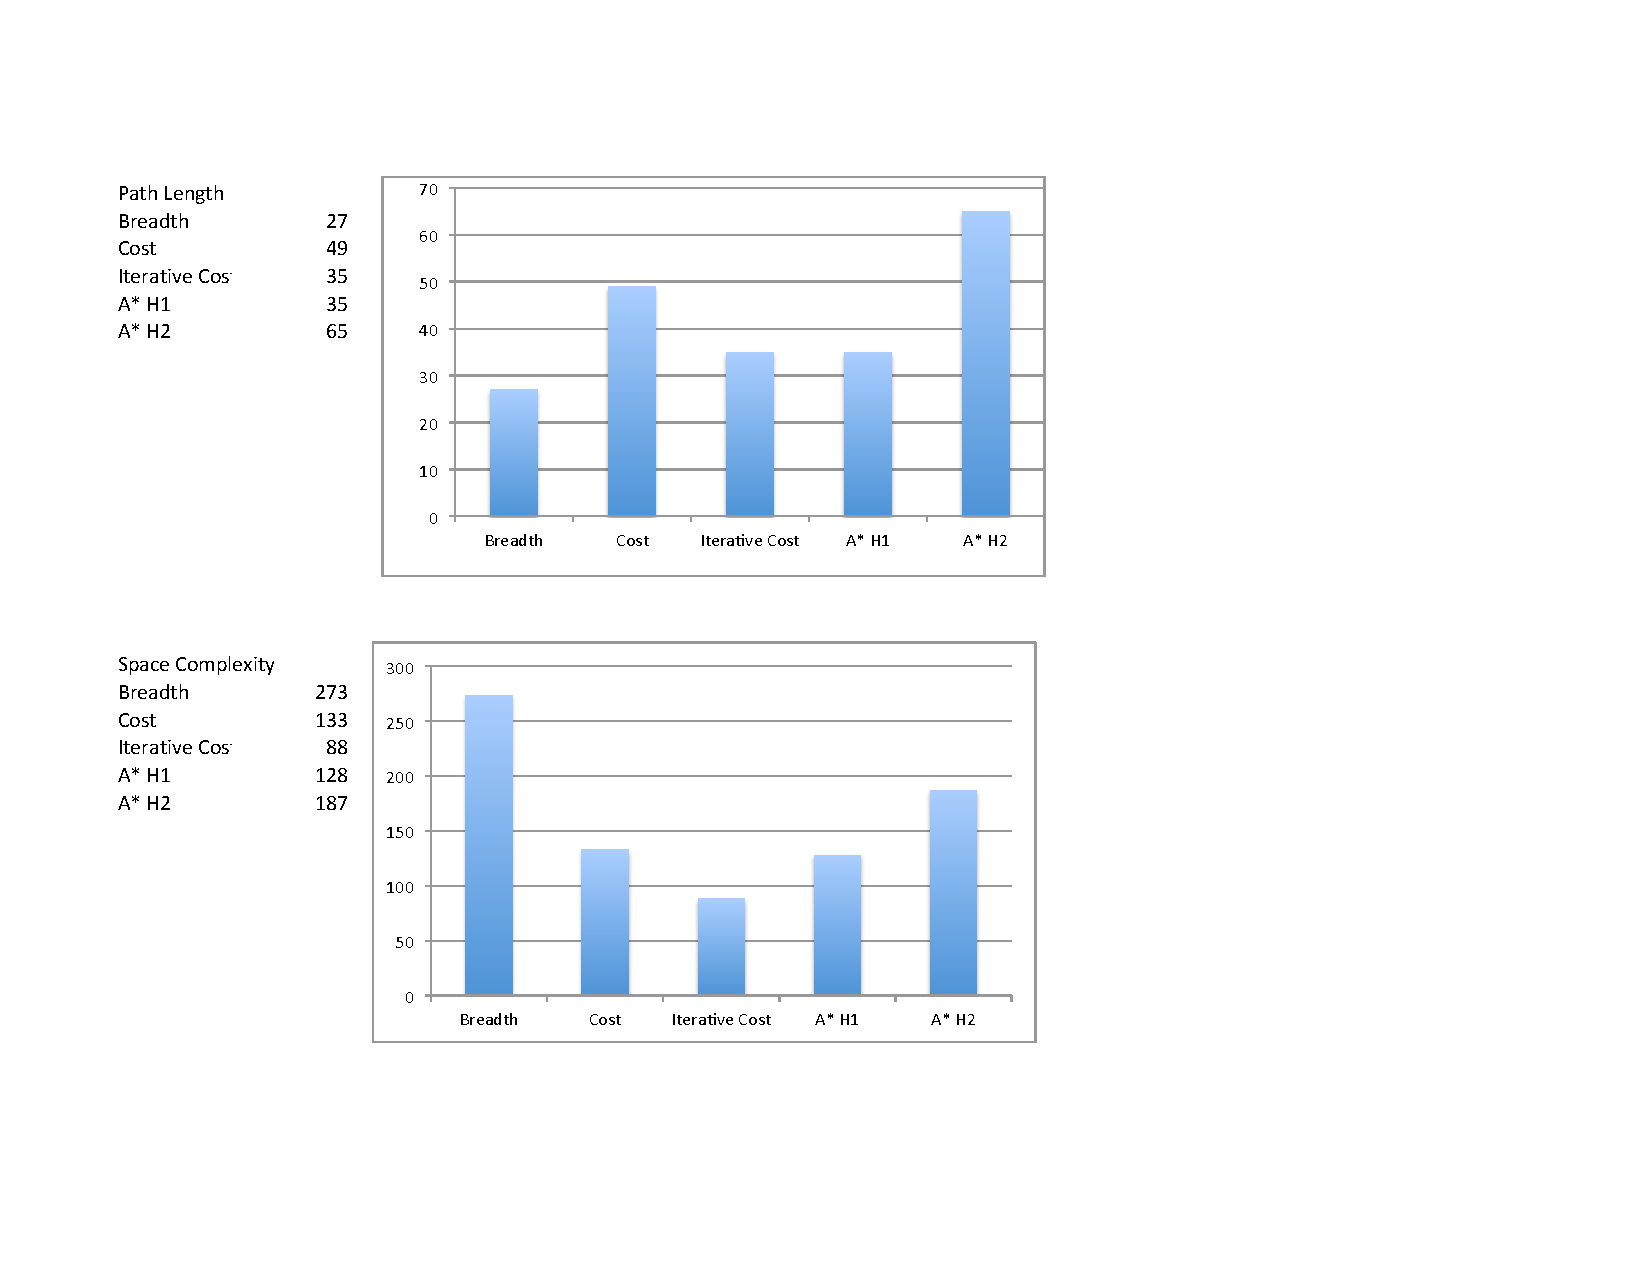
\includegraphics[width=150mm,height=120mm]{images/results2.pdf}
	\end{center}

	From these graphs, Iterative Deepening By Cost Searchfinds has the lowest path cost. But for its slight cost gain, it needs multitudes higher Time Complexity. The next best search is by Lowest Cost. Lowest Cost has still low path cost with low Time Complexity, and has fairly low Space Complexity. After that, A* H1 and H2 have reasonably low path cost, Time and Space Complexity. Breadth First Search only outperforms A*, and has substantially more Space Complexity.


\section{Conclusion}
	From the results, it is clear that if you need a little better path cost, you have to give up a lot of Time Complexity to comute it with Iterative Deepening by Cost. For a little more path cost, one can use Lowest Cost search and have reasonably low Time and Space Complexity. Breadth First Search gets average path cost results with a bit higher Time Complexity, but Space Complexity is considerably higher and expands fast. Which becomes untractable fast with real world problems. A* Heuristics can potentially outperform all searches if well writen, but can fall apart if they are too dependent on certain systems, and revert back to Breadth First Search performance. 
	\\ \\
	In conclusion, pick Iterative Deepening by Cost Search if you have lots of time to find the best path. Otherwise, pick Lowest Cost Search.


\end{document}
